\section{Feynman Diagrams}

\subsection{Exercise}
The first Feynman diagram evaluates to
\begin{equation}
    -i\lambda \int_{-T}^T dtG(t,t)G(t_1,t)G(t_2,t).
\end{equation}
The first diagram in the disconnected set is
\begin{equation}
    (-i\lambda)^2\int_{-T}^T\int_{-T}^T dt'dtG(t_1,t)G(t_2,t)G(t,t')G(t,t')G(t',t_3)G(t',t_4),
\end{equation}
and the second is
\begin{equation}
    -i\lambda \int_{-T}^T dt'' G(t'',t'')G(t'',t'').
\end{equation}
The total disconnected diagram is thus
\begin{equation}
    (-i\lambda)^3\int_{-T}^T\int_{-T}^T\int_{-T}^T dt''dt'dtG(t'',t'')G(t'',t'')G(t_1,t)G(t_2,t)G(t,t')G(t,t')G(t',t_3)G(t',t_4).
\end{equation}
\subsection{Exercise}
The diagrams for 
\begin{equation}
    \bra{0} T\{\hat x_I(t_1)\hat x_I(t_2)\hat x_I(t_3)\hat x_I(t_4)\left(-\frac{i\lambda}{4!}\right)\int_{-T}^T dt \hat x_I^4(t)\}\ket{0}
\end{equation}
are given by all combinations of vertices with 4 external vertices and one internal vertex. These are given by the following:
\begin{center}
    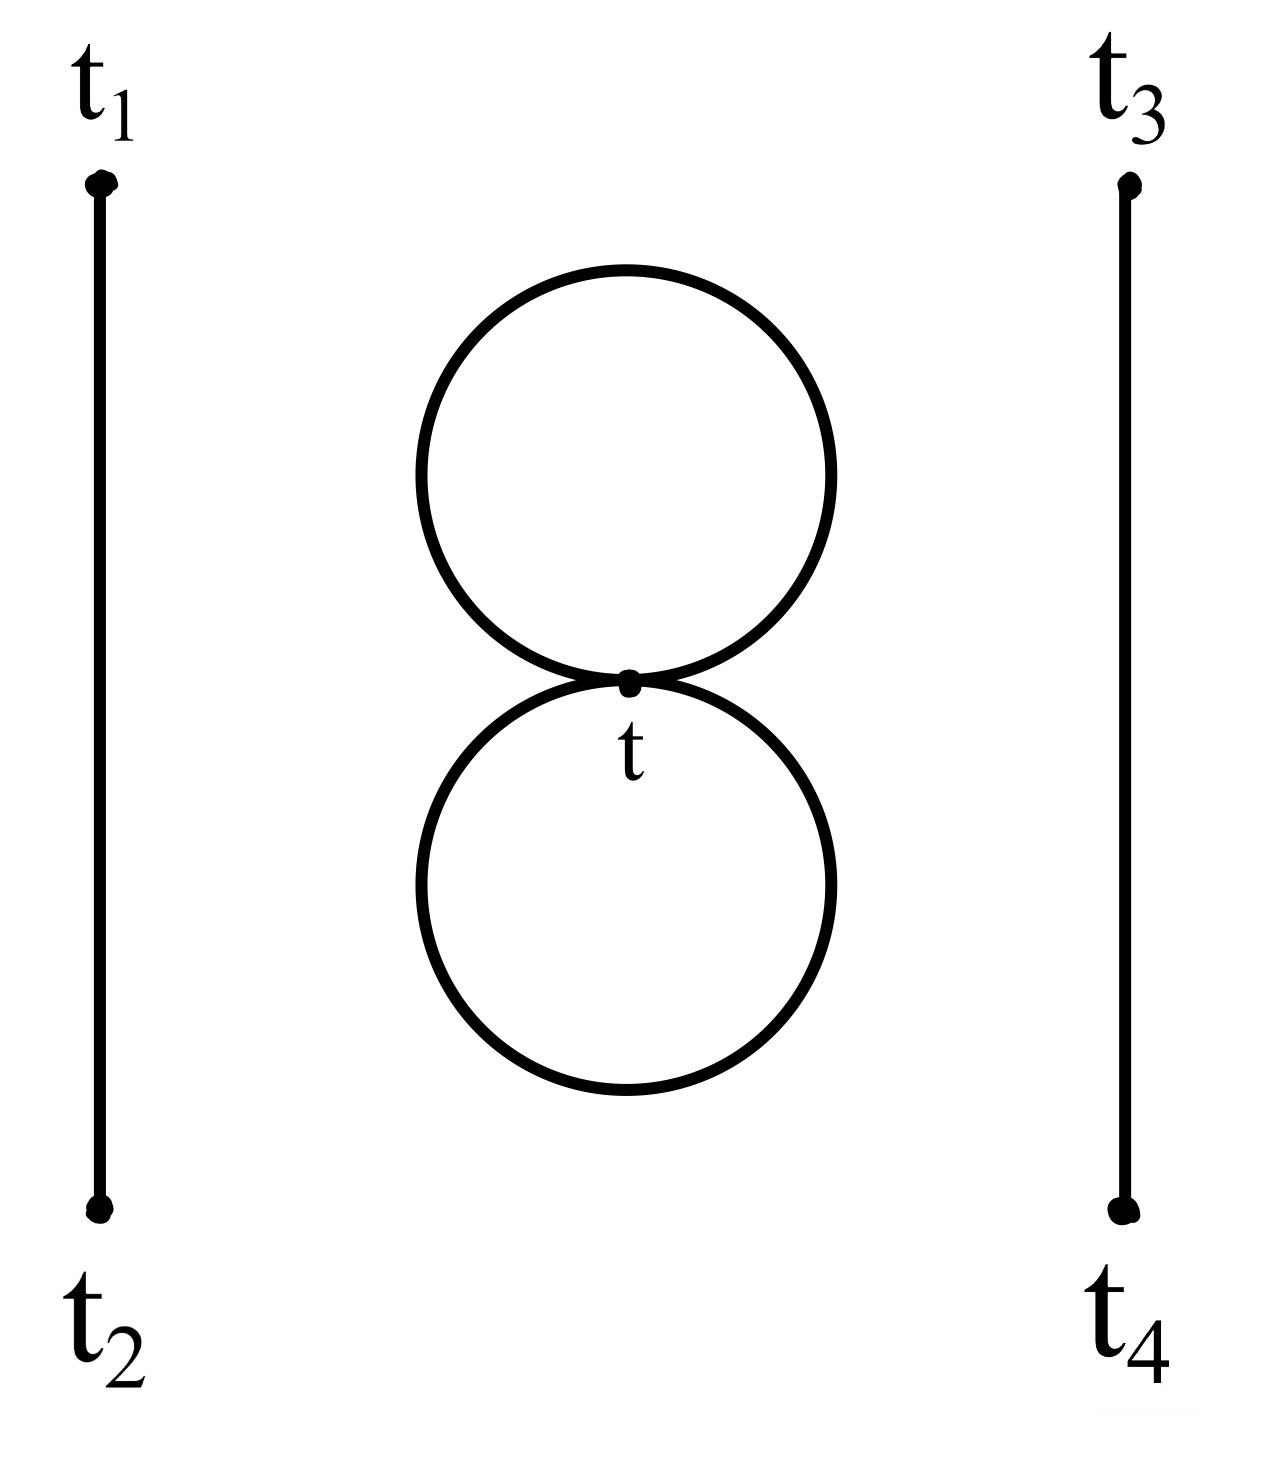
\includegraphics[width=5cm]{sections/IMG_1200.jpeg}
    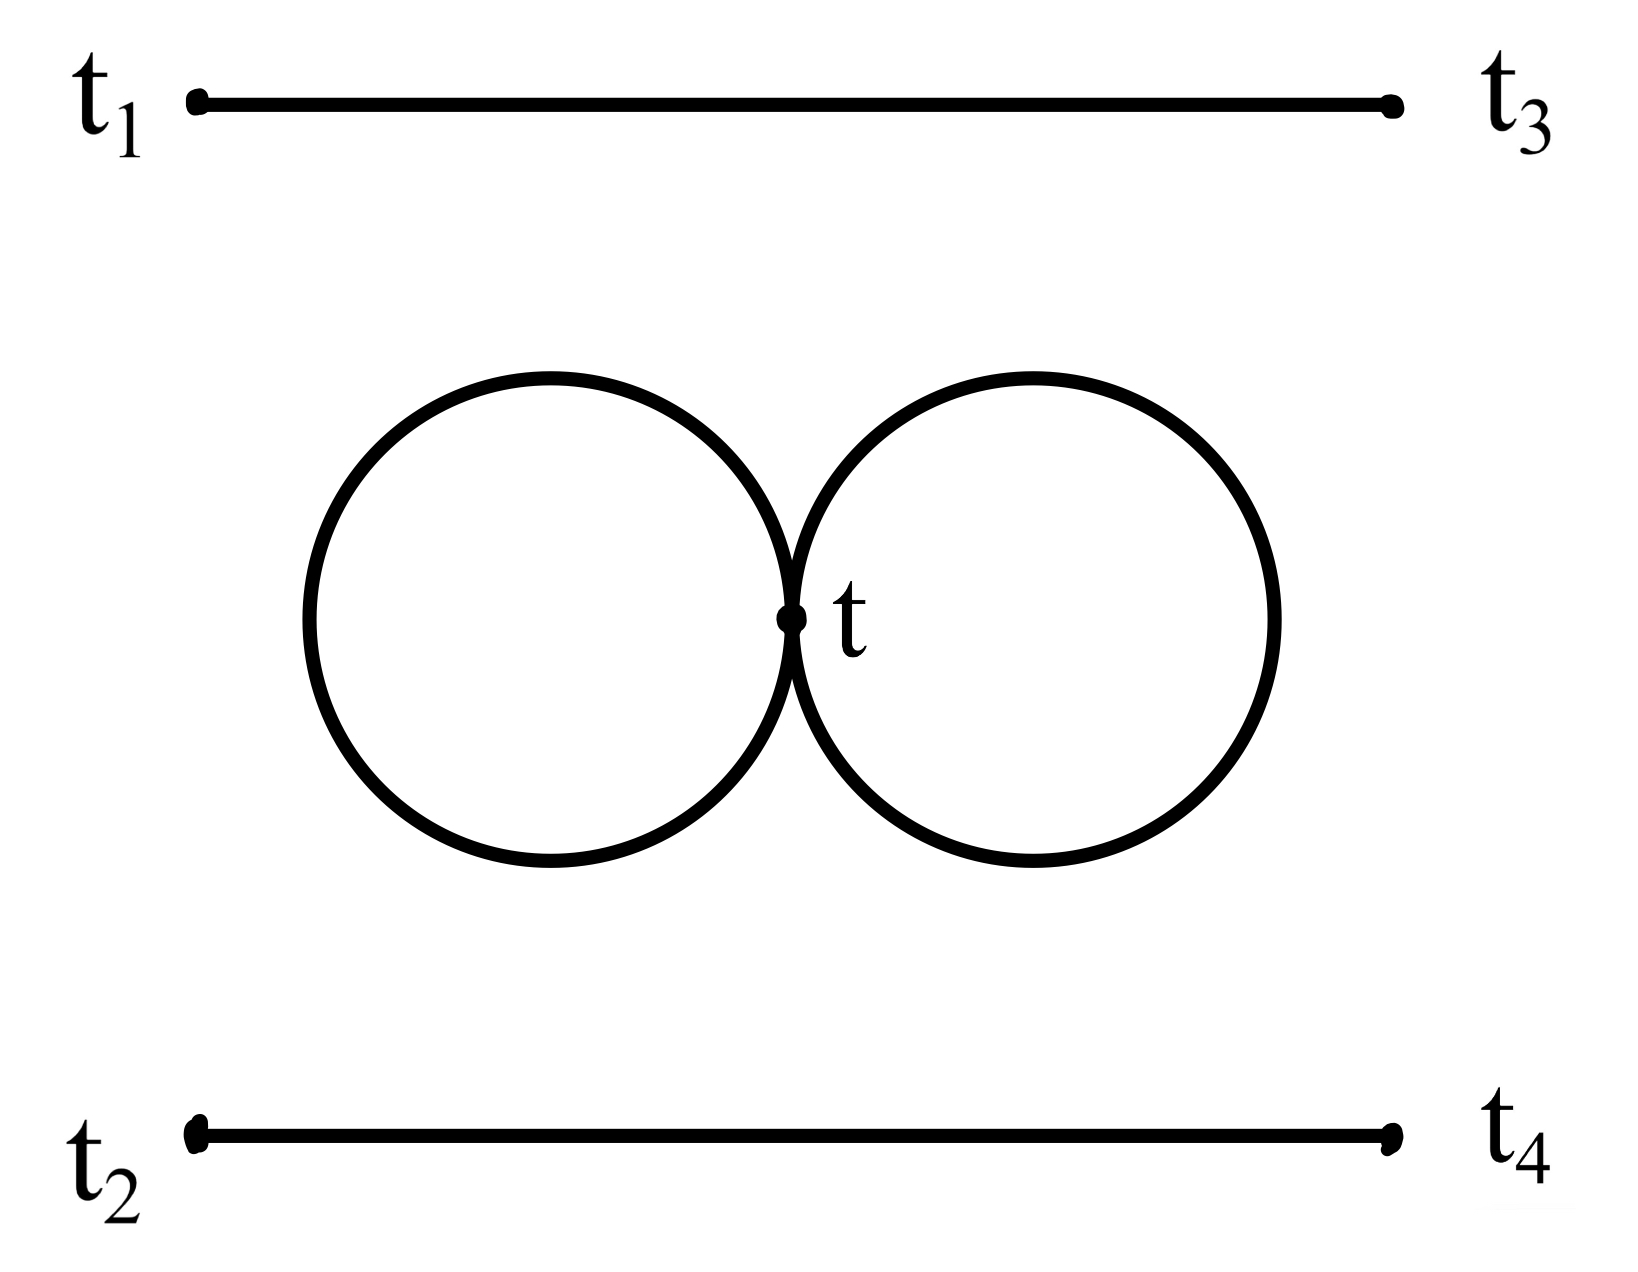
\includegraphics[width=5cm]{sections/IMG_1202.jpeg}
    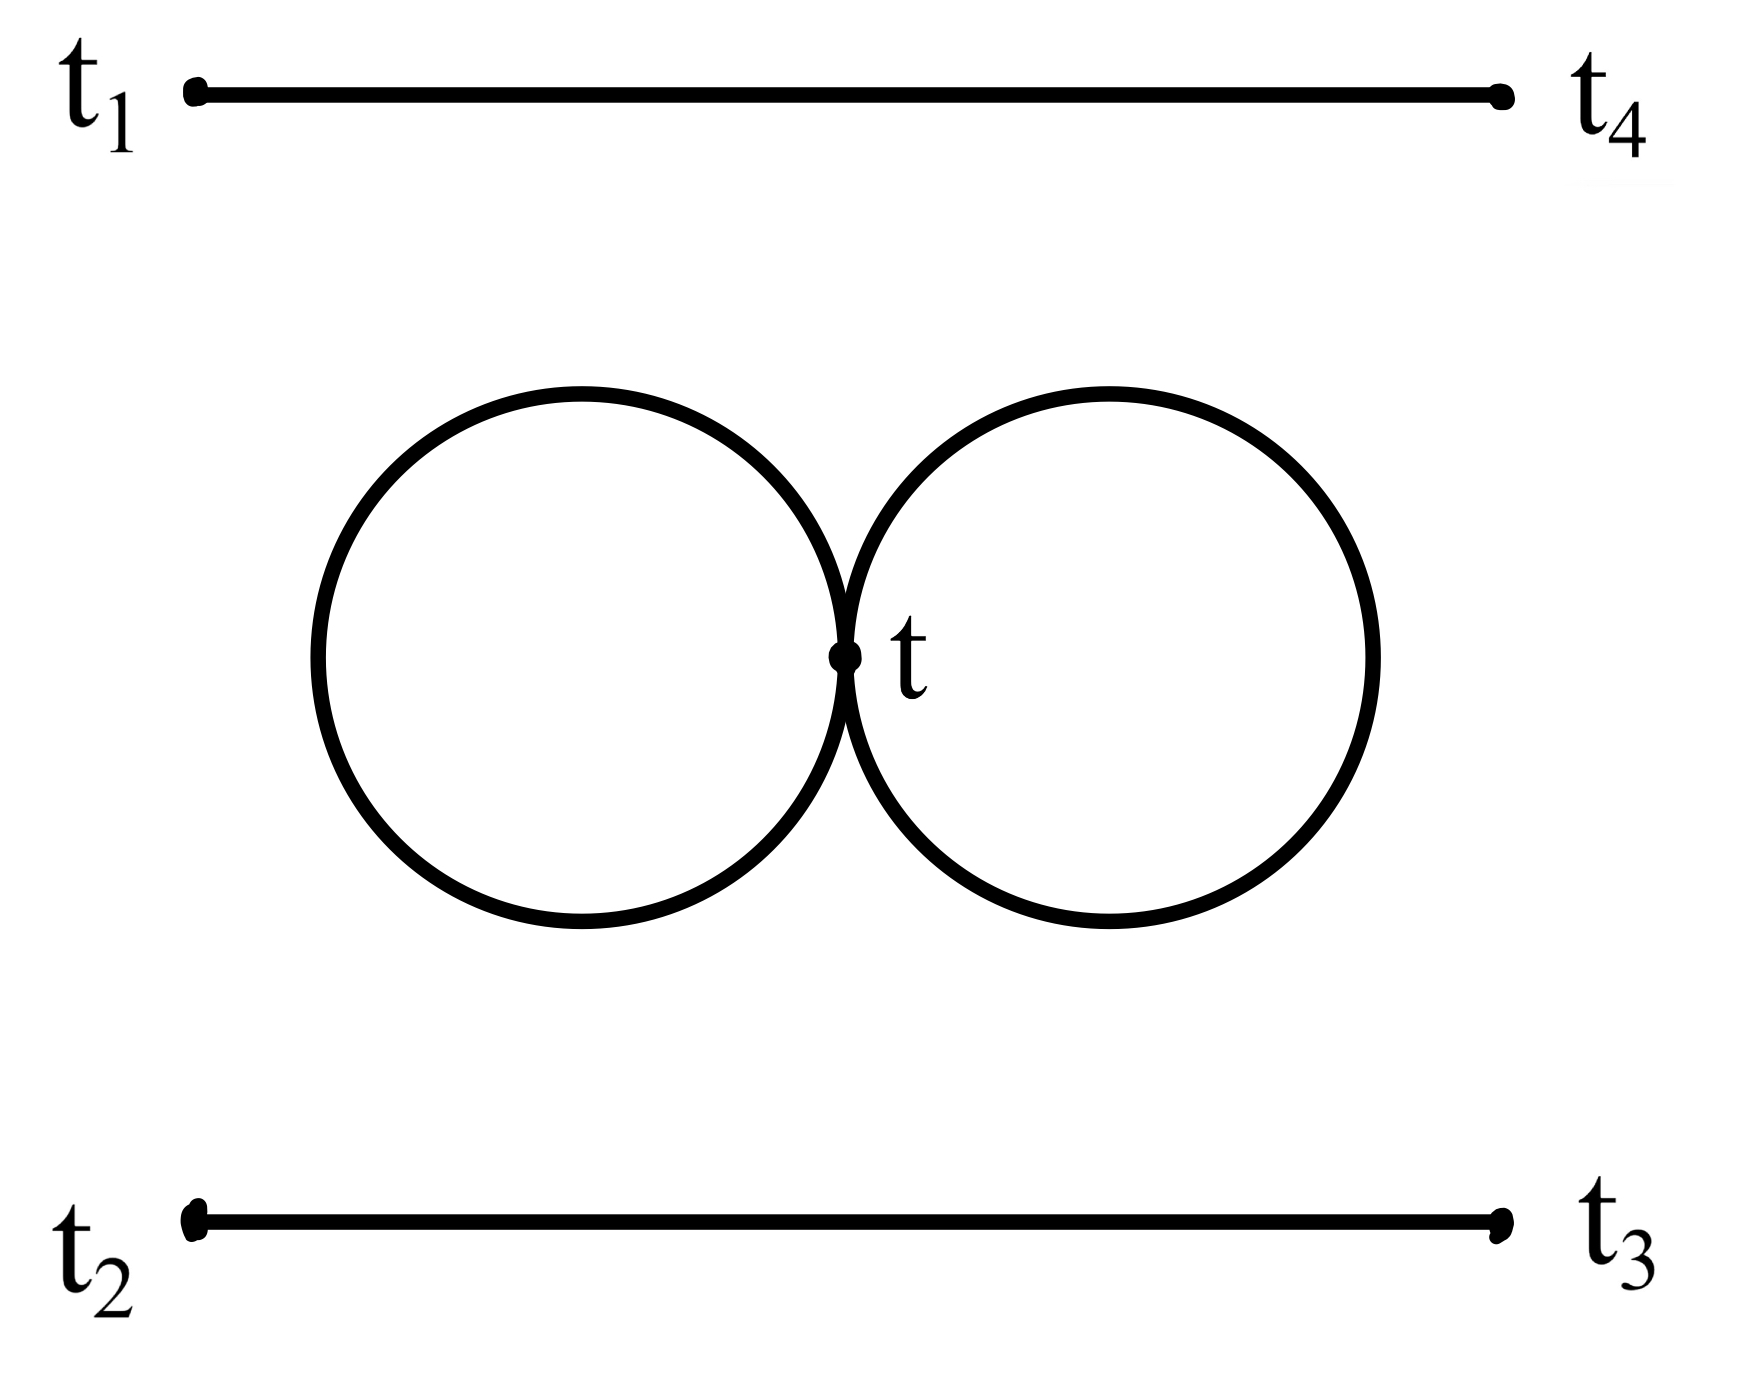
\includegraphics[width=5cm]{sections/IMG_1203.jpeg}
    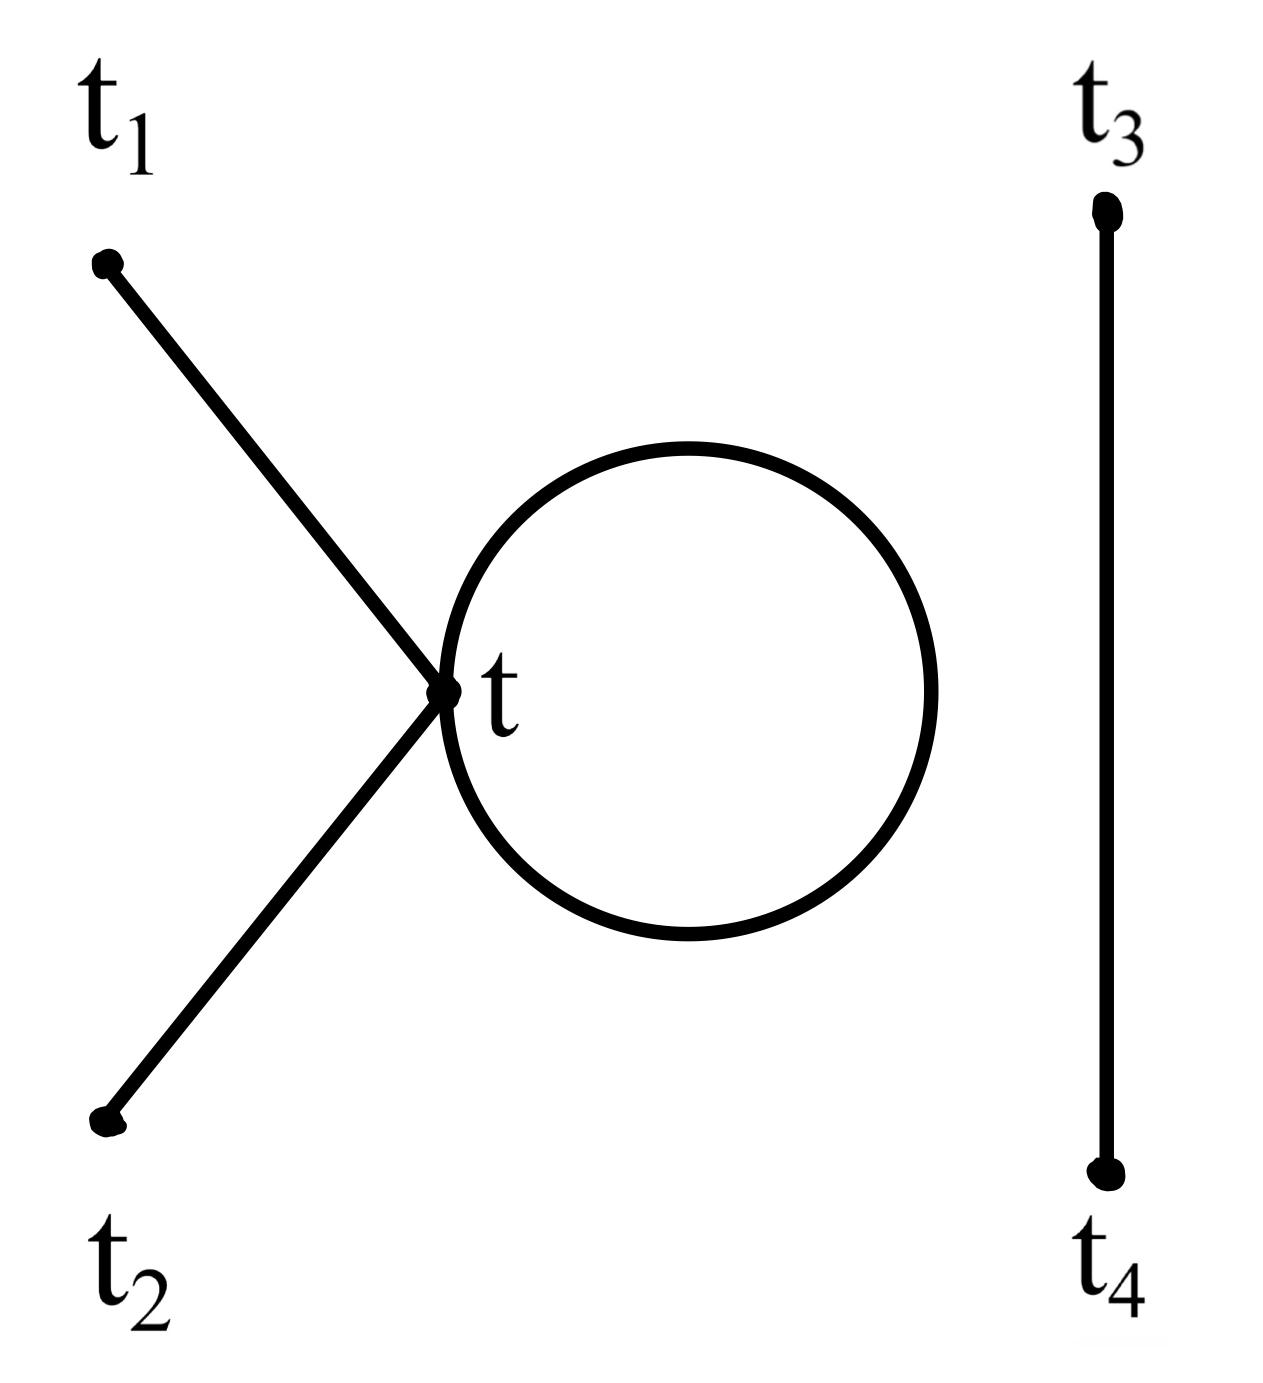
\includegraphics[width=5cm]{sections/IMG_1204.jpeg}
    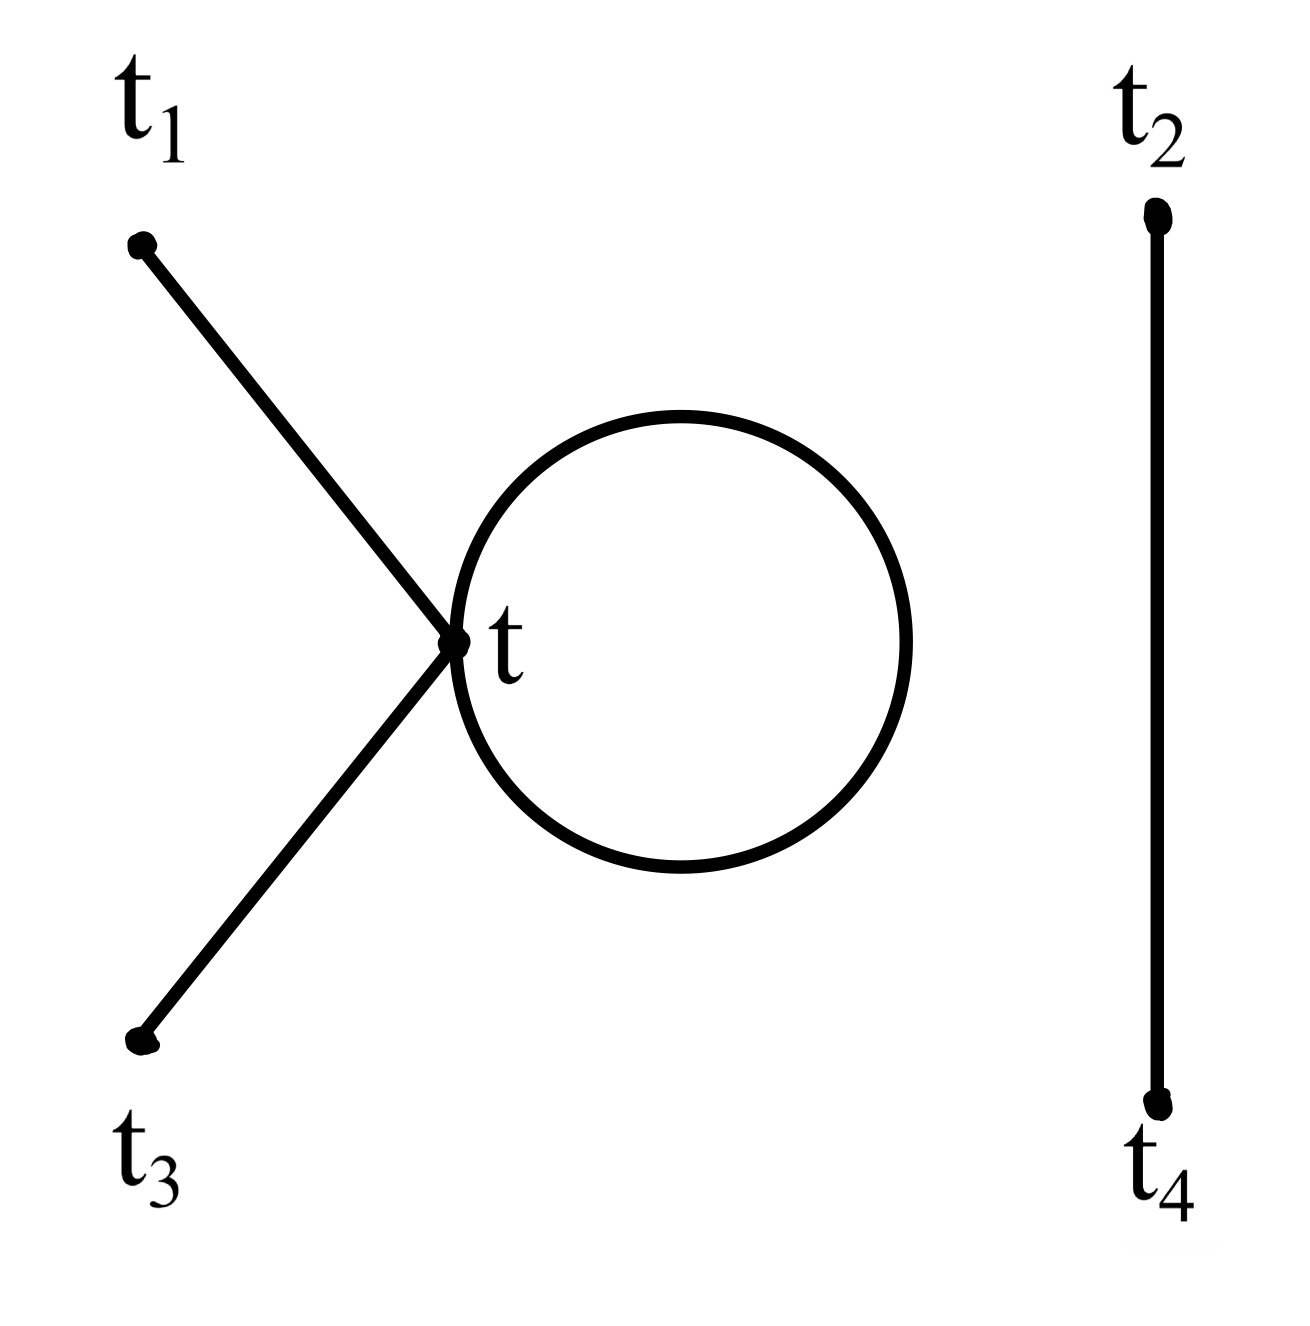
\includegraphics[width=5cm]{sections/IMG_1205.jpeg}
    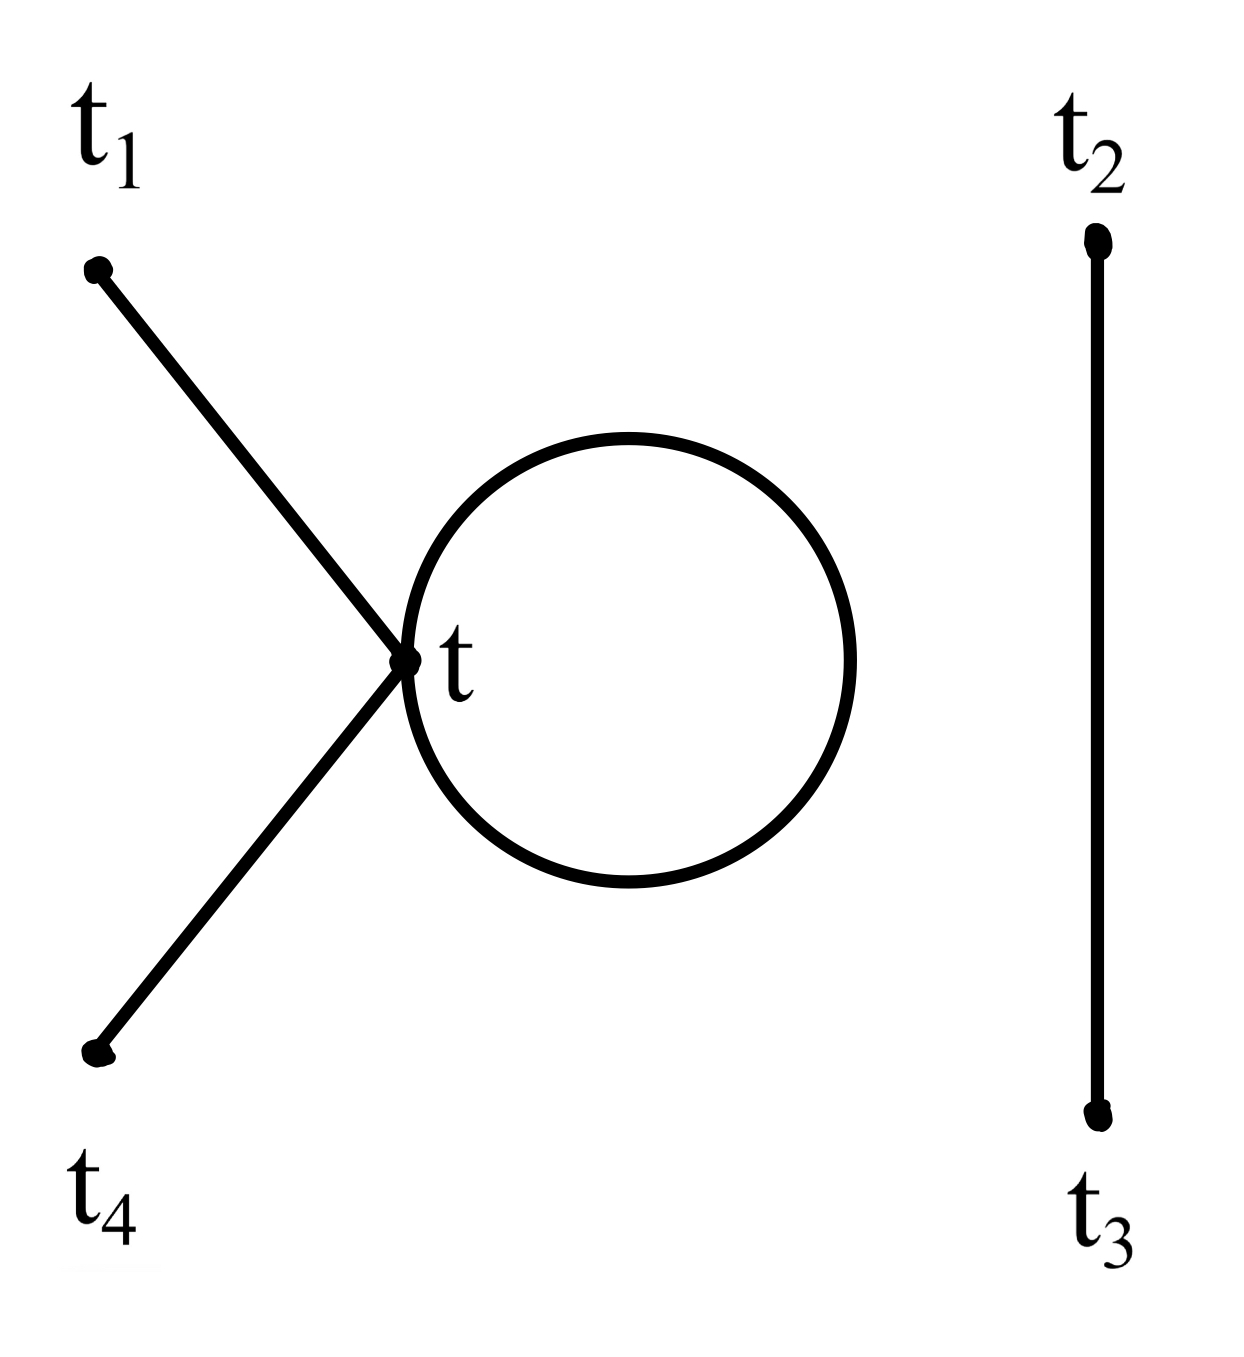
\includegraphics[width=5cm]{sections/IMG_1206.jpeg}
    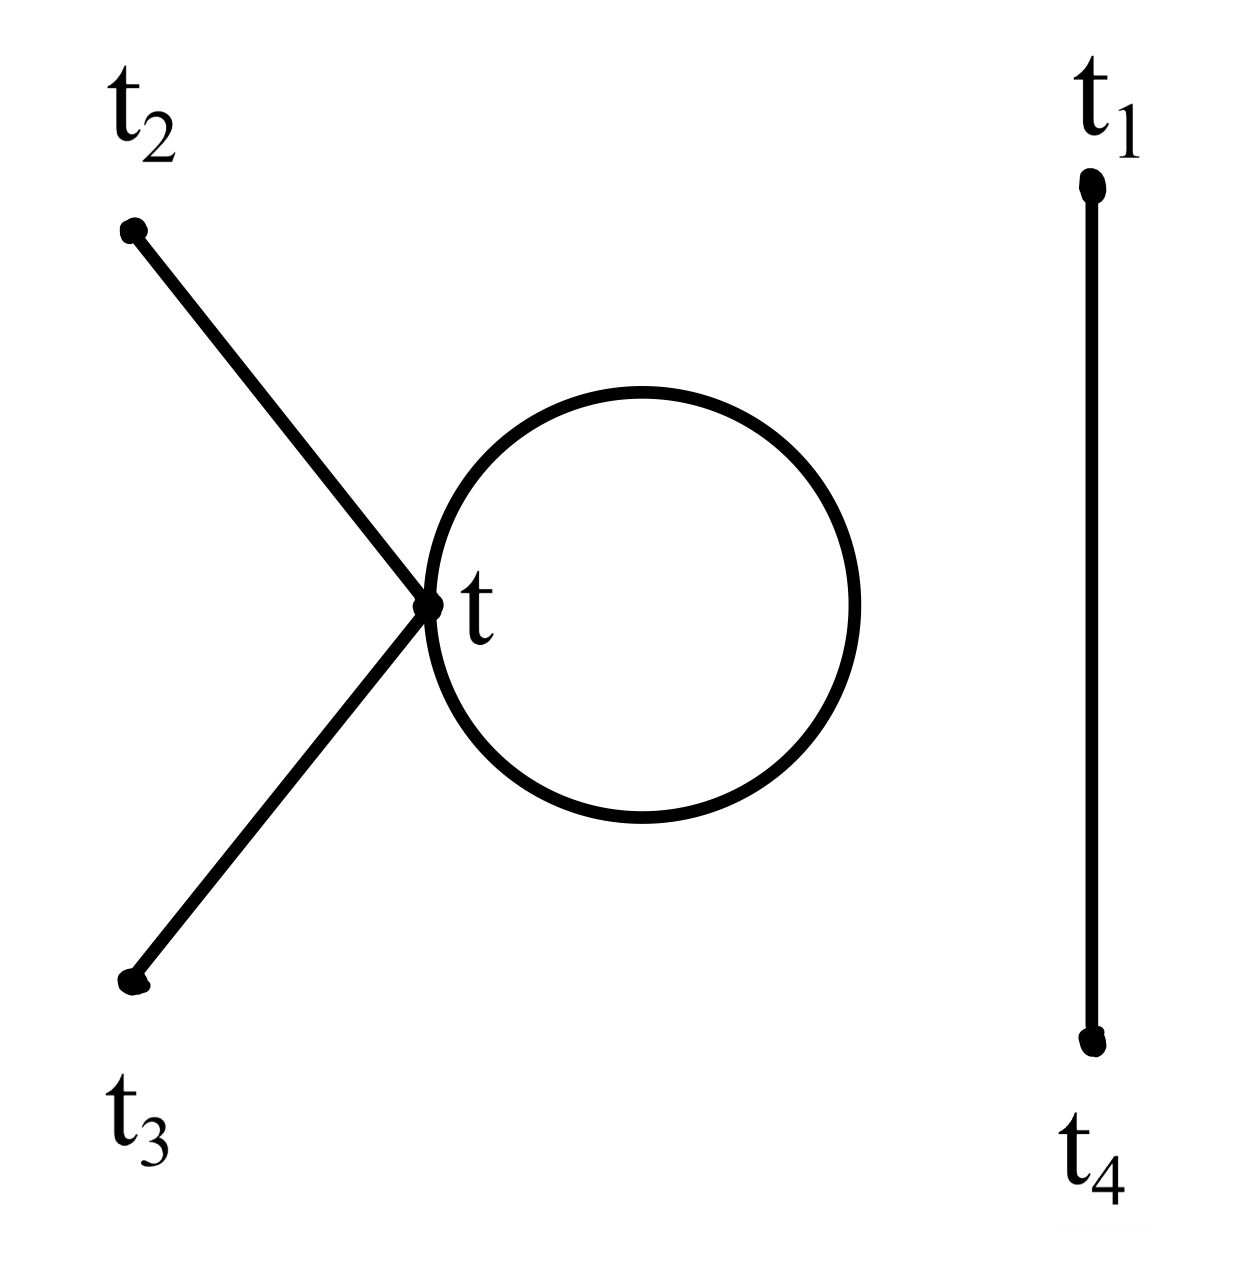
\includegraphics[width=5cm]{sections/IMG_1207.jpeg}
    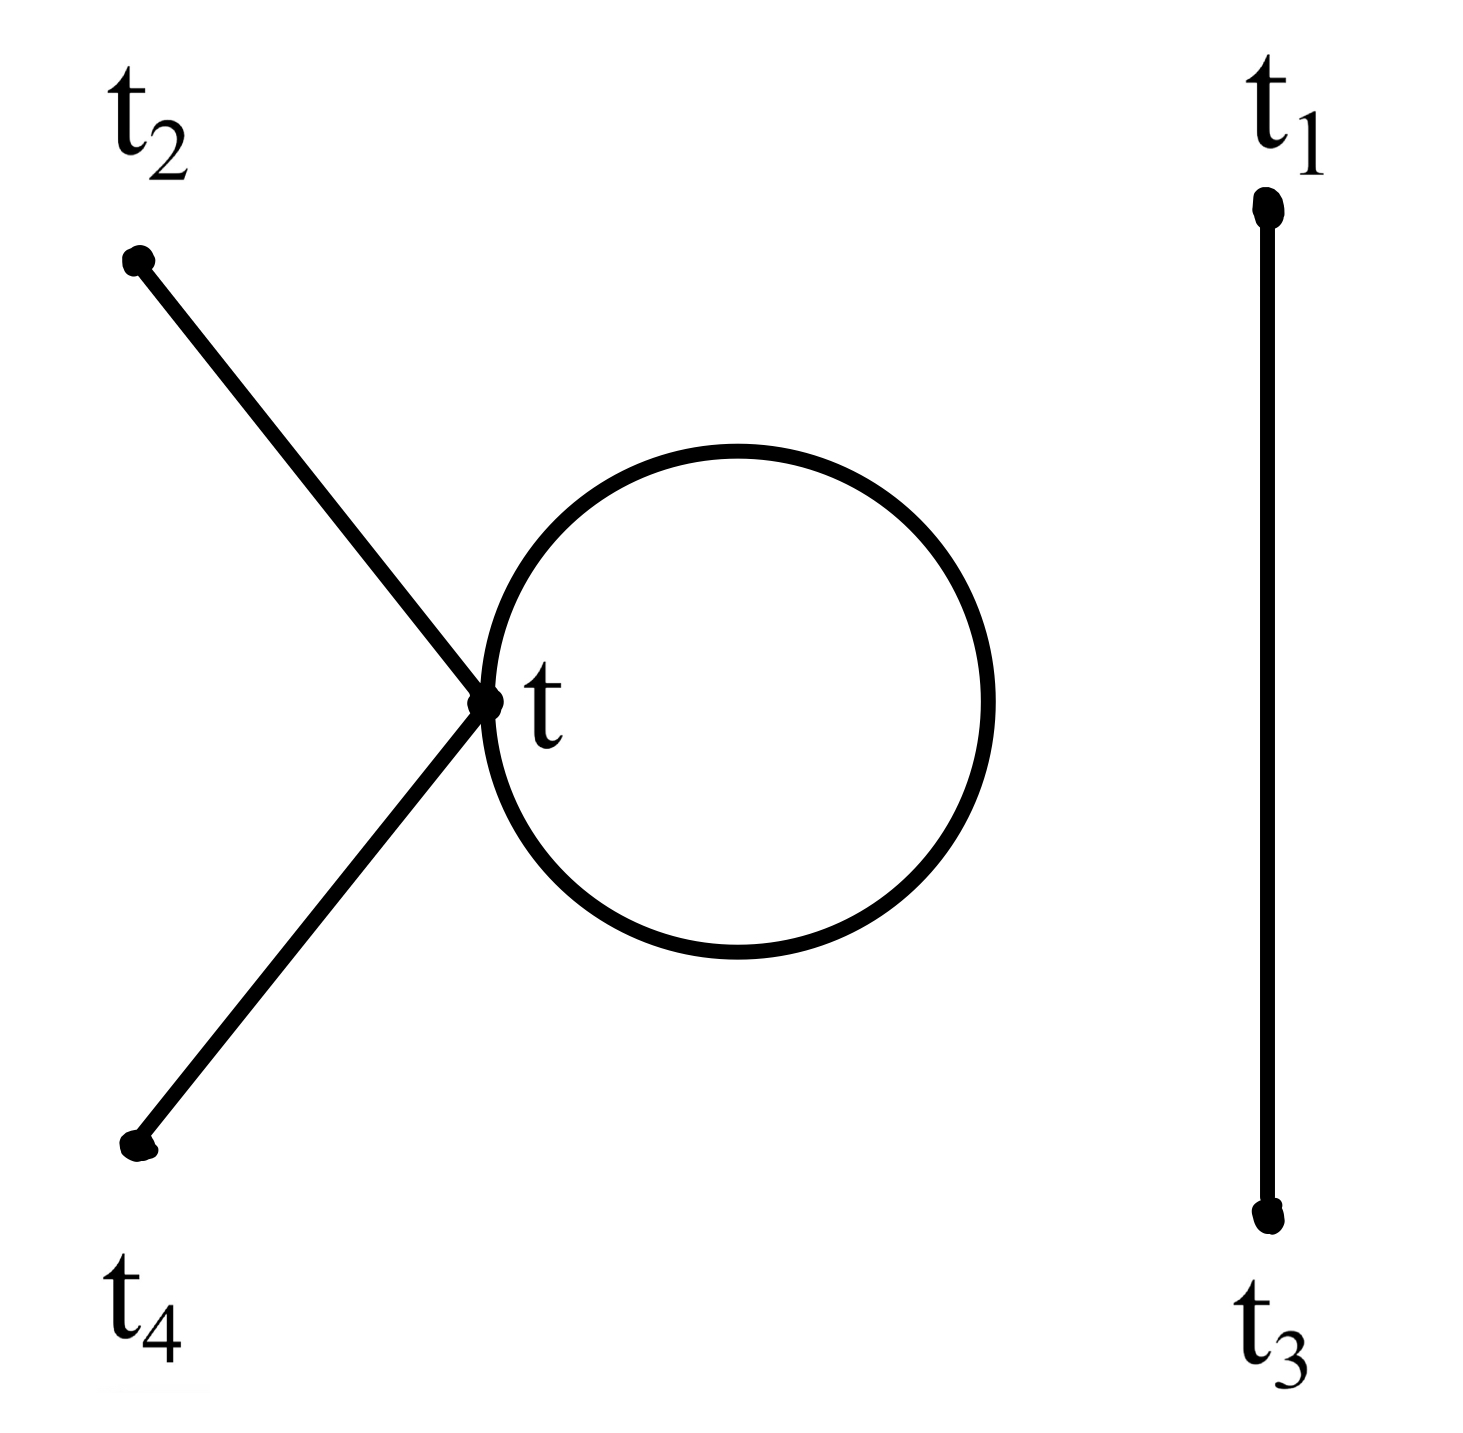
\includegraphics[width=5cm]{sections/IMG_1208.jpeg}
    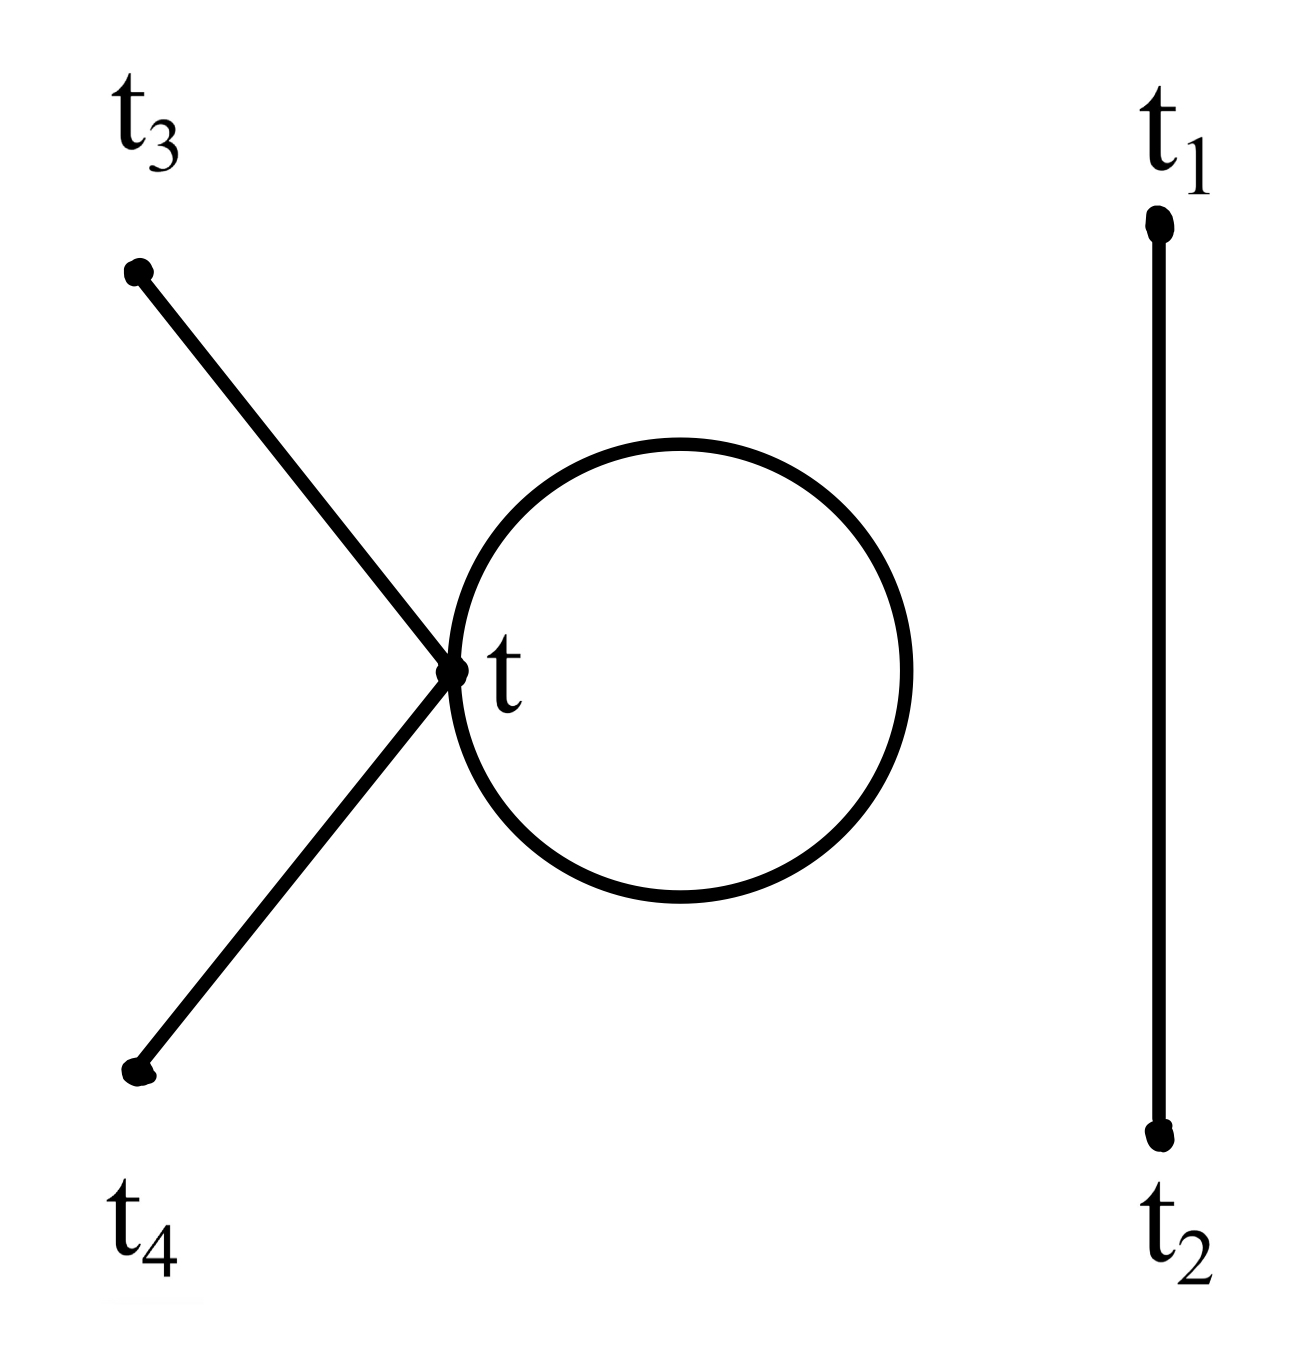
\includegraphics[width=5cm]{sections/IMG_1209.jpeg}
    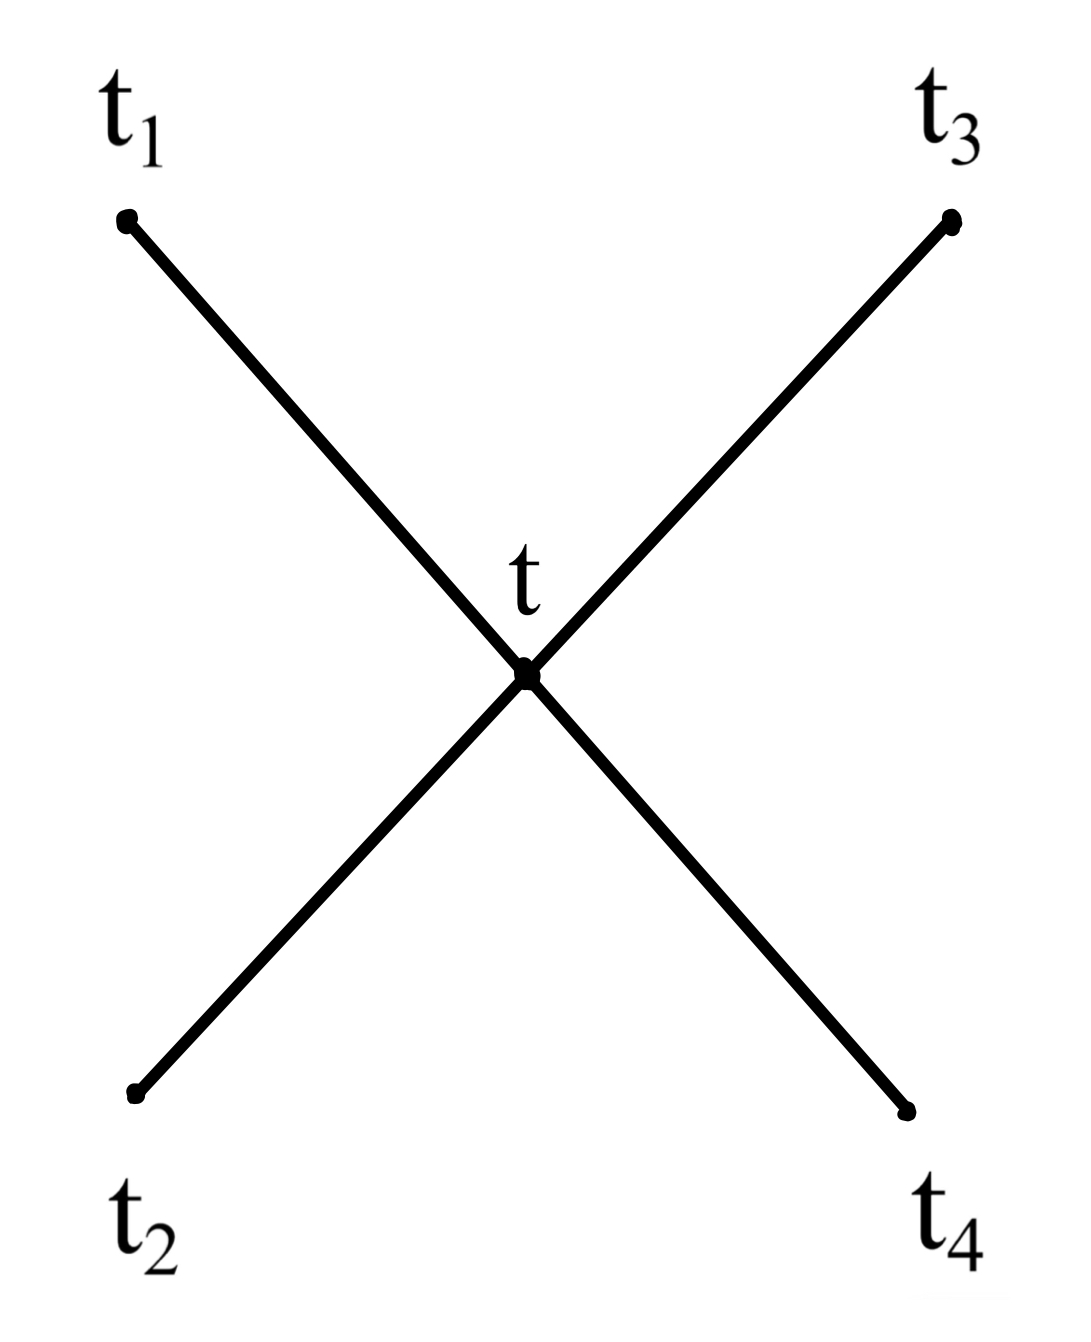
\includegraphics[width=5cm]{sections/IMG_1210.jpeg}
\end{center}
The integrals for the diagrams are given by 
\begin{align}
    D_1=-i\lambda \int dt G(t_1,t_2)G(t_3,t_4)G(t,t)G(t,t) \\
    D_2=-i\lambda \int dt G(t_1,t_3)G(t_2,t_4)G(t,t)G(t,t)\\
    D_3=-i\lambda \int dt G(t_1,t_4)G(t_2,t_3)G(t,t)G(t,t)\\
    D_4=-i\lambda \int dt G(t_1,t)G(t_2,t)G(t,t)G(t_3,t_4)\\
    D_5=-i\lambda \int dt G(t_1,t)G(t_3,t)G(t,t)G(t_2,t_4)\\
    D_6=-i\lambda \int dt G(t_1,t)G(t_4,t)G(t,t)G(t_2,t_3)\\
    D_7=-i\lambda \int dt G(t_2,t)G(t_3,t)G(t,t)G(t_1,t_4)\\
    D_8=-i\lambda \int dt G(t_2,t)G(t_4,t)G(t,t)G(t_1,t_3)\\
    D_9=-i\lambda \int dt G(t_3,t)G(t_4,t)G(t,t)G(t_1,t_2)\\ 
    D_{10}=-i\lambda \int dt G(t_1,t)G(t_2,t)G(t,t_3)G(t,t_4).
\end{align}
Thus, the total contribution of this term will be 
\begin{equation}
    \bra{0} T\{\hat x_I(t_1)\hat x_I(t_2)\hat x_I(t_3)\hat x_I(t_4)\left(-\frac{i\lambda}{4!}\right)\int_{-T}^T dt \hat x_I^4(t)\}\ket{0}=s_1(D_1+D_2+D_3)+s_2(D_4+...+D_9)+s_3D_{10}
\end{equation}
where the $s_i$ are the symmetry factors for each diagram. From the packet, we know $s_1=\frac 3 {4!}=\frac 1 8$. The diagrams $4...9$ all have 1 loop, so $s_2=\frac 2 {4!}=\frac 1 {12}$. The 10th diagram has no loops, so $s_3$ is simply $\frac 1 {4!}=\frac 1 {24}$.


\subsection{Exercise}
Inserting the factors from 9.2, we get 
\begin{align}
    \frac{\bra{0} T\{\hat x_I(t_1)\hat x_I(t_2)\hat x_I(t_3)\hat x_I(t_4)\}\ket{0}+\bra{0} T\{\hat x_I(t_1)\hat x_I(t_2)\hat x_I(t_3)\hat x_I(t_4)\left(-\frac{i\lambda}{4!}\right)\int_{-T}^T dt \hat x_I^4(t)\}\ket{0}}{1-\frac{i\lambda} 8 \int dt G(t,t)G(t,t)}\\
    =\frac{G_{12}G_{34}+G_{13}G_{24}+G_{14}G_{23}+s_1(D_1+D_2+D_3)+s_2(D_4+...+D_9)+s_3D_{10}}{1-\frac{i\lambda} 8 \int dt G(t,t)G(t,t)}.
\end{align}
Using the expansion
\begin{equation}
    \frac 1 {1-x}=1+x+x^2...
\end{equation}
and keeping terms first order in $\lambda$, we get (letting $s_1=\frac 1 8$ and plugging in the expressions for $D_1,D_2$, and $D_3$):
\begin{align}
    &(G_{12}G_{34}+G_{13}G_{24}+G_{14}G_{23}+s_1(D_1+D_2+D_3)+s_2(D_4+...+D_9)+s_3D_{10}...)(1+\frac{i\lambda} 8 \int dt G(t,t)G(t,t)...)\\&=G_{12}G_{34}+G_{13}G_{24}+G_{14}G_{23}\\&+(G_{12}G_{34}+G_{13}G_{24}+G_{14}G_{23})(\frac{i\lambda} 8 \int dt G(t,t)G(t,t))\\&-(G_{12}G_{34}+G_{13}G_{24}+G_{14}G_{23})(\frac{i\lambda} 8 \int dt G(t,t)G(t,t))+s_2(D_4+...+D_9)+s_3D_{10}).
\end{align}
Noting that the second and third terms cancel, we are left with
\begin{equation}
    G_{12}G_{34}+G_{13}G_{24}+G_{14}G_{23}+s_2(D_4+...+D_9)+s_3D_{10}.
\end{equation}

\subsection{Exercise}
The integral for this diagram is
\begin{equation}
    -i\lambda \int_{-T}^TdtG(t_1,t)G(t_2,t)G(t,t).
\end{equation}
Using the Green's function for a harmonic oscillator, 
\begin{equation}
    G(t_2,t_1)=\frac 1 {2\omega} e^{-i\omega |t_2-t_1|},
\end{equation}
this is 
\begin{equation}
    -i\lambda\int_{-T}^T \frac {dt}{(2\omega)^3}e^{-i\omega(|t_1-t|+|t_2-t|+|t-t|)}. 
\end{equation}
Inserting $t_1=t_2=0$, this simplifies to 
\begin{equation}
     -i\lambda \int_{-T}^T \frac{dt}{(2\omega)^3} e^{-2\omega i |t|}=-\frac{i\lambda}{(2\omega^3)}\left[2\int_0^T dt e^{-2\omega i t}\right]
\end{equation}
because the integrand is even in $t$. This integral can be evaluated as
\begin{equation}
    -\frac{i\lambda}{(2\omega)^3}\frac 2 {-2\omega i}\left[e^{-2\omega i T}-1\right]= -\frac{2\lambda}{(2\omega)^4}\left[1-e^{-2\omega i T}\right].
\end{equation}
In the limit $T \to \infty (1 - i\epsilon)$, the second term becomes
\begin{equation}
    \lim_{T \to \infty (1 - i\epsilon)}e^{-2\omega i T}=e^{-2\omega i \infty}e^{-2\omega \epsilon \infty}=0
\end{equation}
when $\epsilon>0$, and since the first term always has magnitude 1. Then the diagram evaluates to 
\begin{equation}
    -\frac{2\lambda}{(2\omega)^4}=-\frac{\lambda}{8\omega^4}.
\end{equation}